\chapter{Symmetrische Authentifikation von Nachrichten}
\label{cha:symauth}

Bisher haben wir uns nur mit der Frage beschäftigt, wie ein
Kommunikationsteilnehmer Bob eine Nachricht an Alice für einen
unbefugten Lauscher unverständlich machen, also verschlüsseln kann. Wir
haben uns noch nicht der Frage nach der Authentifikation einer Nachricht
gewidmet.  Der Angreifer könnte mit dem entsprechenden Zugriff auf den
Übertragungskanal sogar eine verschlüsselte Kommunikation beeinflussen,
deren Inhalt er nicht versteht. Er kann Nachrichten abfangen, verändern
und wieder auf den Weg bringen, ohne dass Alice oder Bob etwas von dem
Zwischenstopp der Nachricht bemerken.  Falls ein Angreifer trotz der
Verschlüsselungsmaßnahmen außerdem in der Lage ist, die Kommunikation zu
verstehen, könnte er sogar \textit{gezielt} den Inhalt von Nachrichten
verändern.  Es kann jedoch auch ohne Angreifer geschehen, dass der
Kommunikationskanal gestört und Bobs Nachricht durch technische
Einwirkungen abgewandelt wird.

Im besten Fall erhält Alice dann eine unbrauchbare Nachricht und kann
bei Bob eine Wiederholung anfordern. Im schlechtesten Fall ist die
Veränderung zufällig (oder vom Angreifer gewollt) sinnvoll und
beeinflusst damit das weitere Vorgehen der beiden
Kommunikationsteilnehmer.

\section{Ziel} Angesichts dessen, dass wir uns unseren
Kommunikationskanal nicht immer aussuchen können, hätten wir gern einen
Mechanismus, der uns ermöglicht, eine erhaltene Nachricht auf Fehler und
Veränderungen zu überprüfen (Integrität) und den Absender zu bestimmen
(Authentizität). Dafür erstellt Bob für seine Nachricht $M$ zusätzlich
eine "`Unterschrift"' $\sigma$ und überträgt diese gemeinsam mit
$M$. Alice erhält das Paar $(M,\sigma)$ und überprüft, ob die
Unterschrift auf die erhaltene Nachricht passt.

Um ein funktionierendes und gegen einen PPT-Angreifer möglichst sicheres
Unterschriftensystem zu erhalten, müssen einige Anforderungen erfüllt
sein:
\begin{itemize}
\item Bob muss $\sigma$ aus der bzw. für die Nachricht $M$ berechnen
  können.
\item Alice muss $\sigma$ zusammen mit $M$ verifizieren können.
\item ein PPT-Angreifer soll kein gültiges $\sigma$ für ein selbst
  gewähltes $M$ berechnen können.
\end{itemize}

\section{MACs}
\label{ch:symauth:macs} 
\textit{Message Authentication Codes} (MACs) sind ein symmetrisches
Verfahren, um die Authentizität einer Nachricht sicherzustellen. Hierzu
gibt es einen Signatur- und einen Verifikationsalgorithmus. Beide
Algorithmen sind PPT-Algoritmen und verwenden als Eingabe ein
gemeinsames Geheimnis $K$: 

\begin{itemize}
\item \textbf{Signieren:} $\sigma \leftarrow \sig(\key,\plaint)$.
\item \textbf{Verifizieren:} $\ver(\key,\plaint,\sigma) \in \{0,1\}$.
\end{itemize} 
\subsubsection*{Korrektheit}
Ein MAC-Verfahren heißt \textit{korrekt}, wenn gilt:
\[
\forall \plaint~\forall \key: \ver(\key, \plaint, \sig(\key, \plaint)) =1.
\]
$\ver$ gibt also $1$ zurück, wenn $\sigma$ mit der übertragenen
Nachricht und  dem korrekten Geheimnis $\key$ erzeugt wurde.

Analog zu symmetrischen Verschlüsselungsverfahren ist $\key$ für gewöhnlich
ein zufällig gewählter Bit-String.
\section{Der EUF-CMA-Sicherheitsbegriff}
\label{ch:symauth:sicherheit} Damit ein MAC uns nicht nur vor
Übertragungsfehlern, sondern auch vor einem Angreifer schützt, verlangen
wir, dass kein PPT-Angreifer ein MAC fälschen, also selbstständig ein Nachrichten-Signatur-Paar
finden kann, das gültig ist.

Er bekommt dafür ein Signaturorakel mit vor ihm verborgenem Schlüssel
$K$, mit dem er Nachrichten seiner Wahl signieren kann. Er gewinnt, wenn
er die Signatur einer Nachricht $\plaint$ korrekt vorhersagen kann, ohne $\plaint$
vorher an das Orakel gegeben zu haben. Etwas strukturierter sieht der
Angriff für einen PPT-Angreifer \A~so aus:
\begin{enumerate}
\item \A~erhält Zugriff auf ein Signaturorakel
  $\sig(\key,\cdot)$, an dass er polyomiell viele Nachrichten $\plaint_i$
  schicken darf (in beliebiger Reihenfolge und unabhängig von einander)
  und jeweils $\sigma_i$ mit $\ver(\key, \plaint_i, \sigma_i)=1$ als Antwort erhält.
\item \A~gibt als (potentielle) Fälschung ein Nachrichten-Signatur-Paar
  $(\plaint^*,\sigma^*)$ aus.
\item \A~gewinnt, wenn $\sigma^*$ eine gültige Signatur für
  $\plaint^*$ ist, d.h. $\ver(\key, \plaint^*, \sigma^* = 1)$, und $\plaint^*
  \neq \plaint_i$ für alle $i$ ist, d.h. $\plaint^*$ nicht zu den
  Nachrichten gehört, die sich \A~vom Orakel hat signieren lassen.
\end{enumerate} 

Ein MAC (\sig, \ver) ist \textit{EUF-CMA-sicher\footnote{\textit{EUF} steht für
    \textit{Existential Unforgeability}. Damit ist gemeint, dass es
    keine Nachricht geben darf, für die ein PPT-Angreifer \A~eine
    Fälschung erstellen kann. \A~ darf sich also selbst aussuchen, zu
    welcher Nachricht er eine Signatur fälscht. \textit{CMA}
    steht für \textit{adaptiv Chosen Message Attack}. Damit ist ausgedrückt,
    dass dem Angreifer nicht vorgeschrieben wird, welche Nachrichten er
    sich vom Orakel signieren lässt. Insbesondere darf er seine Anfragen
    von bereits erhaltenen $\plaint_i$, $\sigma_i$ abhängig machen.}},falls jeder
PPT-Algoritmus \A~das obigen Spiel nur mit (im Sicherheitsparameter $k$)
vernachlässigbarer Wahrscheinlichkeit gewinnt.

Abbildung \ref{fig:euf-cma} zeigt dieses Sicherheitsexperiment noch
einmal grafisch.49

Dieser Sicherheitsbegriff bildet passive Angriffe ab, bei denen der
Angreifer keinen Zugriff auf die $\ver$-Funktion hat, sondern "`blind"'
signiert. In vielen Fällen ist dieser Sicherheitsbegriff aber äquivalent
zu dem, bei dem der Angreifer Zugriff auf ein \ver-Orakel erhält,
beispielsweise wenn es für jede Nachricht \plaint~nur eine einzige (also
eindeutige) gültige Signatur $\sigma$ gibt. Die Hauptidee um diese
Äquivalenz zu zeigen ist die folgende: Gibt der Angreifer die
Signaturen, die er von seinem \sig-Orakel erhält, an sein \ver-Orakel
weiter, so erhält er keine neue Information (da die Signatur vom Orakel
kommt, kann er sich bereits sicher sein, dass sie gültig ist). Würde er
aber ein Nachrichten-Signatur-Paar finden, zudem das Ver-Orakel $1$
ausgibt und das er nicht vom Sig-Orakel erhalten hat, so könnte er
dieses auch bereits als seine Fälschung ausgeben und müsste das
\ver-Orakel gar nicht verwenden.

\begin{center} 
\begin{figure}
  \scalebox{1.2}{
    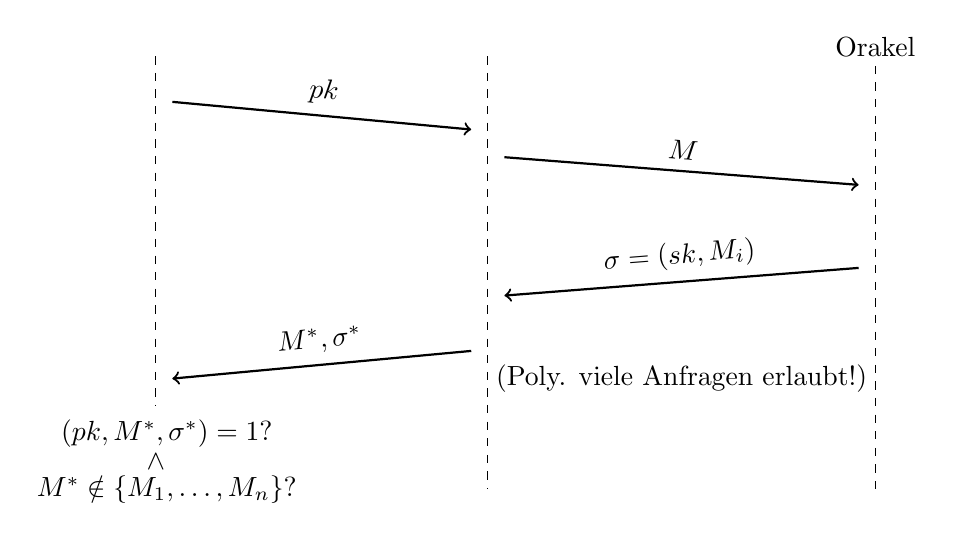
\begin{tikzpicture}[x=2em, y=2em]
      \draw (-6,0) node (C) {$\C$}; 
      \draw (0,0) node (A) {$\A$}; 
      \draw (7,0) node (Ork) {Orakel};
      
      \draw[dashed] (C) -- (-6,-6.5);
      \draw[dashed] (A) -- (0,-8);
      \draw[dashed] (Ork) -- (7,-8);
      
      \textbf{\draw[->, thick] (-5.7,-1) -- (-0.3,-1.5)
        node[sloped,above,pos=0.5] {$pk$}; 
      }
      \textbf{\draw[->, thick] (0.3,-2) -- (6.7,-2.5)
        node[sloped,above,pos=0.5] {$M$};}
      \textbf{\draw[->, thick] (6.7,-4) -- (0.3,-4.5)
        node[sloped,above,pos=0.5] {$\sigma = \sig(sk, M_i)$};}

      \draw (3.5,-6) node (exp) {(Poly. viele Anfragen erlaubt!)};
      
      \textbf{\draw[->, thick] (-0.3, -5.5) -- (-5.7,-6)
        node[sloped,above,pos=0.5] {$M^*, \sigma^*$};}
      
      \draw (-5.8,-7) node (b2) {$\ver(pk, M^*, \sigma^*) = 1$?};
      \draw (-6,-7.5) node (b3) {$\wedge$};
      \draw (-5.8,-8) node (b4) {$M^* \notin \{M_1, \dots, M_n\}$?};
    \end{tikzpicture}
  }
  \caption{Ablauf des EUF-CMA-Experimentes}
  \label{fig:euf-cma}
\end{figure}
\end{center}

\section{Konstruktionen}

\subsection{Hash-then-Sign Paradigma} 
Viele Signaturverfahren können nur Nachrichten fester Länge
signieren. Für praktische Anwendungen wollen wir aber meist Nachrichten
beliebiger Länge signieren können. Hierzu bieten sich Hash-Funktionen an, die
Nachrichten beliebiger Länge auf einen Bit-String fester Länge abbilden.

Die Idee des \emph{Hash-then-Sign} Paradigmas ist also, anstelle der
vollständigen Nachricht $M~\in~\{0,1\}^*$ den aus ihr berechneten
Hashwert $H(M) \in \{0,1\}^k$ zu signieren. Die
Sicherheit des MACs ist dabei sowohl von der verwendeten Hashfunktion
als auch vom Signaturalgorithmus abhängig.~\\

% Die Idee des \emph{Hash-then-Sign} Paradigmas ist also, nicht die
% vollständige Nachricht $M~\in~\{0,1\}^*$ zu signieren, sondern den aus
% dieser Nachricht berechneten Hashwert $H(M) \in \{0,1\}^k$. Die
% Sicherheit des MACs ist dabei sowohl von der verwendeten Hashfunktion
% als auch vom Signaturalgorithmus abhängig.~\\

\begin{theorem} Sei $(\sig, \ver)$ EUF-CMA-sicher und $H$ eine
  kollisionsresistente Hashfunktion. Dann ist der durch
  \begin{align*} 
    \sig'(K,M) &= \sig(K,H(M))\\ 
    \ver'(K,M,\sigma) &= \ver(K,H(M),\sigma)
  \end{align*} erklärte MAC EUF-CMA-sicher.~\\
\end{theorem}

\begin{beweisidee}
  \label{ch:symauth:eufcma-beweis}
Der  EUF-CMA-Angreifer \A~hat zwei Möglichkeiten. Er kann direkt eine
Signatur $\sigma$ für eine Nachricht \plaint~fälschen. Dies steht aber
im Widerspruch zur vorrausgesetzen EUF-CMA-Sicherheit von $(\sig,
\ver)$, da dann $(H(\plaint), \sigma)$ eine gültige Fälschung für dieses
Schema wäre. Somit kann \A~nur eine im Sicherheitsparameter $k$ vernachlässigbare
Erfolgswahrscheinlichkeit haben. Die zweite Möglichkeit ist, dass er vom
Orakel eine Signatur $\sigma'$ für eine Nachricht $\plaint'$ anfragt und
eine andere Nachricht $\plaint^* \neq \plaint'$ findet, sodass
$\ver'(H^*, \sigma') = \ver(H(\plaint^*), \sigma') = 1$. Aus der
EUF-CMA-Sicherheit von $(\sig,\ver)$ folg aber direkt, dass dafür
$H(\plaint') = H(\plaint^*)$ gelten muss (Ansonsten wäre $(H(\plaint^*,
\sigma'))$ eine gültige Fälschung für $(\sig, \ver)$). D.h. \A~müsste
also eine Kollision berechnen, was er aufgrund der Kollisionsresistenz
der Hashfunktion ebenfalls nur mit in $k$ vernachlässigbarer
Erfolgswahrscheinlichkeit kann. Insgesamt folgt die Behauptung.
\end{beweisidee}

\subsection{Pseudorandomisierte Funktionen}\label{ssec:prf} Wenn man
sich die Berechnung eines MACs als eine einfache Funktion im
mathematischen Sinne vorstellt und damit die Errechnung eines
"`frischen"' MACs zum Finden eines unbekannten Funktionswertes wird,
erkennt man schnell, dass Regelmäßigkeit in einer solchen Funktion zu
Sicherheitslücken führt. Zielführender ist es, die Funktionswerte
möglichst zufällig auf ihre Urbilder zu verteilen.
\begin{definition}[Pseudorandomisierte Funktion (PRF)] Sei  \[\text{\textit{PRF}}\colon\{0,1\}^k \times \{0, 1\}^k \rightarrow
  \{0,1\}^k\] eine über $k \in \mathbbm{N}$ parametrisierte Funktion. $PRF$
  heißt Pseudorandom Function (PRF), falls für jeden PPT-Algorithmus
  $\mathcal{A}$ die Funktion
  \begin{equation*} \text{Adv}_{\text{\textit{PRF}},\mathcal{A}}^{prf}(k)
    := \Pr \lbrack \mathcal{A}^{\text{\textit{PRF}}(K,\cdot)}(1^k) = 1
    \rbrack - \Pr \lbrack \mathcal{A}^{R(\cdot)}(1^k) = 1 \rbrack
  \end{equation*} vernachlässigbar im Sicherheitsparameter $k$ ist, wobei $R: \{0,1\}^k \rightarrow
  \{0,1\}^k$ eine echt zufällige Funktion ist.~\\
\end{definition}

Ein Kandidat für eine solche PRF ist eine Hash-Konstruktion: $PRF(K,X) =
H(K,X)$. Allerdings lässt sich eine solche Konstruktion manchmal, wie
bereits in Abschnitt \ref{ch:hash:merkledamgard} bei Merkle-Damgård
ausgenutzt, nach der Berechnung von $H(K,X)$ auch ohne Zugriff auf das
Geheimnis $K$ noch auf $H(K,X,X')$ erweitern. Das führt dazu, dass die
PRF-Eigenschaft für Eingaben unterschiedlicher Länge nicht mehr
hält. Abbildung \ref{fig:symauth:prf} verdeutlicht das.

\begin{figure}[h]
  \begin{center} \unitlength=1mm \linethickness{0.4pt} \hspace{-3 cm}
    \begin{picture}(70,40)

      \put(10,27){\vector(1,0){15}} \put(17,28){\makebox(0,0)[cb]{IV}}

      \put(30,37){\vector(0,-1){7.5}} \put(33,31){\makebox(0,0)[cb]{$K$}}

      \put(25,24.5){\framebox(10,5){$F$}}

      \put(35,27){\vector(1,0){12}} \put(52,37){\vector(0,-1){7.5}}
      \put(55,31){\makebox(0,0)[cb]{$X$}}

      \put(47,24.5){\framebox(10,5){$F$}}

      \put(57,27){\vector(1,0){8}} \put(75,25){\makebox(0,0)[cb]{$H(K,X)$}}


      \put(0,10){\vector(1,0){15}} \put(7,11){\makebox(0,0)[cb]{IV}}

      \put(20,20){\vector(0,-1){7.5}} \put(23,15){\makebox(0,0)[cb]{$K$}}

      \put(15,7.5){\framebox(10,5){$F$}}

      \put(25,10){\vector(1,0){12}} \put(42,20){\vector(0,-1){7.5}}
      \put(45,15){\makebox(0,0)[cb]{$X$}}

      \put(37,7.5){\framebox(10,5){$F$}}

      \put(47,10){\vector(1,0){12}} \put(64,20){\vector(0,-1){7.5}}
      \put(67,15){\makebox(0,0)[cb]{$X'$}}

      \put(59,7.5){\framebox(10,5){$F$}}

      \put(69,10){\vector(1,0){8}} \put(89,8){\makebox(0,0)[cb]{$H(K,X,X')$}}

      \put(53,4){\makebox(0,0)[cb]{\Large{$\Uparrow$}}}
      \put(53,-2){\makebox(0,0)[cb]{$H(K,X)$ bekannt}}

    \end{picture}
  \end{center}
  \caption{\emph{Merkle-Damgård}-Konstruktion $H_{MD}$. Es ist möglich, an
    einen bereits bekannten Hashwert $H(K,X)$ einen Wert $X'$ anzuhängen und
    trotzdem einen korrekten Hashwert zu erzeugen.}
  \label{fig:symauth:prf}
\end{figure}

Als nächstes wollen wir untersuchen, wie aus einer PRF und einer
kollisionsresistenten Hashfunktion ein EUF-CMA-sicherer MAC Konstruiert
werden kann. 
Dazu sei
\begin{align*}
\sig(K,M): \sigma &\leftarrow \text{\textit{PRF}}(K,H(M)) \\
\ver(\sigma, M): & 1 \Leftrightarrow \sigma \stackrel{?}{=}\text{\textit{PRF}}(K,H(M)).
\end{align*}

\begin{theorem} Sei $\text{PRF}\colon\{0,1\}^k \times \{0,1\}^k
  \rightarrow \{0,1\}^k$ eine PRF und $H \colon \{0,1\}^* \rightarrow
  \{0,1\}^k$ eine kollisionsresistente Hashfunktion.  Dann ist der oben
  definierte MAC EUF-CMA-sicher.
\end{theorem} \vspace{10pt}

\begin{beweis}[Entwurf] Sei $\mathcal{A}$ ein erfolgreicher
  EUF-CMA-Angreifer auf ein durch $\sig(K,M) =
  \text{\textit{PRF}}(K,H(M))$ gegebenen MAC. Dann können wir annehmen,
  dass $\mathcal{A}$ eine Fälschung $(M^*,\sigma^*)$ mit einer noch nicht
  signierten Nachricht $M^*$ berechnen kann. Wir können also $\mathcal{A}$
  als \textit{PRF}-Unterscheider auffassen, der mit
  nicht-vernachlässigbarer Wahrscheinlichkeit
  $\text{\textit{PRF}}(K,H(M^*))$ vorhersagt. Eine Vorhersage ist jedoch
  nur dann möglich, wenn \textit{PRF} keinen Zufall ausgibt. Da
  \textit{PRF} jedoch nach Definition nur mit im Sicherheitsparameter $k$ vernachlässigbarer
  Wahrscheinlichkeit von echtem Zufall unterscheidbar ist, kann es einen
  solchen \textit{PRF}-Unterscheider nicht geben.
\end{beweis}

\subsection{HMAC} In Abschnitt \ref{ssec:prf} zu
\hyperref[ssec:prf]{pseudorandomisierten Funktionen}
haben wir gesehen, dass Signaturverfahren, dass Hashfunktionen, die auf
Merkle-Damgård basieren, beim Einsatz in Signaturverfahren für Probleme
führen können. Insbesondere sind sie bezüglich der EUF-CMA-Sicherheit
problematisch.  Ein Angreifer, dem $\sigma = H(K,M)$ bekannt ist, erhält
durch Anfügen eines Blockes $X$ problemlos den korrekten Hashwert
$H(K,M,X)$ und somit die Signatur der Nachricht $M,X$.  Dennoch ist es
möglich, EUF-CMA-sichere MACs zu konstruieren, die die Hashfunktionen
verwenden, die auf der Merkle-Damgård-Konstruktion basieren. Eines der verbreitetsten
Verfahren ist der \textit{Keyed-Hash Message Authentication Code}, der
HMAC. Das Signieren einer Nachricht funktioniert dabei wie folgt:
\begin{equation*}
  \sig(K,M) = H(K \oplus \textit{opad}, H(K \oplus
  \textit{ipad}, M))
\end{equation*}
Um eine Signatur zu prüfen, erstellt der Empfänger selbst eine Signatur
und prüft, ob diese mit der erhaltenen Signatur übereinstimmt.
Dabei sind \textit{opad}, das \textit{outer padding},
und \textit{ipad}, das \textit{inner padding}, zwei Konstanten der
Blocklänge $m$ der Hashfunktion, die bei jedem Signaturvorgang gleich
bleiben. Üblich\footnote{Sowohl im RFC 2104, sowie in einer
  Veröffentlichung des NIST und in diverser Fachliteratur werden diese
  Werte (als Standard) vorgeschlagen. Siehe: ~\\~\\
  \url{http://tools.ietf.org/html/rfc2104} \\
  \url{http://csrc.nist.gov/publications/fips/fips198-1/FIPS-198-1_final.pdf}}
ist es, $opad = \{0x5C\}^{m/8}$ und $ipad = \{0x36\}^{m/8}$ zu
wählen. 

Immun gegen den in Abbildung \ref{fig:symauth:prf} vorgestellten Angriff
ist HMAC aufgrund seiner verschachtelten Struktur. Die Nachricht $M$,
die es zu Signieren gilt, wird in jeweils zwei Hash\-vorgängen
verarbeitet. Für eine Nachricht $M,X$ ist
\begin{equation*}
 H(K \oplus \textit{opad}, H(K \oplus \textit{ipad}, M), X)
\end{equation*} 
aber offensichtlich keine gültige Signatur. Der
Angreifer müsste einen Nachrichtenblock $X$ bereits im inneren
Hashvorgang unterbringen. Da er dafür allerdings $H$ invertieren, oder
das Geheimnis $K$ kennen müsste, schlägt der Angriff fehl.